\documentclass[10pt]{article}
\usepackage{icmlko}

\icmlmeta{IP 파운데이션 월드모델}{125}{라벨을 섞자 정렬이 사라졌다}{판정치가 방법을 전제하고 있었다 --- 하네스를 방법에서 떼어내자 첫 라운드에서 챔피언이 바뀌었다}

\begin{document}

\twocolumn[
\icmlheader

\begin{abstract}
스물여덟 노트 동안 한 정식화 안에서만 움직였다. 노트 103에서 ``구조적
막다른 골목''이라 적어 놓고도 그 안에서 스무 편을 더 돌았다. 이번에 그
기제를 찾았다. \textbf{판정치가 방법을 전제한 정의였다.} 앙상블 판정치는
``출처마다 예측을 받아 순위 평균''이라 적혀 있었고, 그것은 \emph{쌍별 정렬
후 전이}가 있다고 가정한 문장이다. 그래서 최적수송이든 파운데이션
in-context든 확산 모형이든 \textbf{점수를 매길 수가 없었다.} 대안이 경쟁에
못 들어오면 남는 일은 현행을 손보는 것뿐이다. 그래서 정식화에 요구하는 것을
하나로 줄인 하네스를 짰다 --- (도메인, 축, 마스크, 시간)에서 점수 벡터로,
순위만 의미. 여기에 상시 가드 여섯과 챔피언/도전자 루프, 별도 서버의 모니터를
붙였다. \textbf{첫 라운드에서 챔피언이 바뀌었다.} 정렬을 아예 안 하고 전
도메인을 한 표에 쌓은 뒤 도메인 표시자만 준 F6이 판 $\rho$ $+$0.3413,
프로크루스테스가 $+$0.3400 --- 원점수로는 무승부다. \textbf{그런데 가드가
둘을 갈랐다.} 출처 라벨을 도메인마다 섞고 99번 다시 적합한 귀무 분포에서
F6은 폭 0.127, F1은 0.178이다. 표준화하면 $+$2.84$\sigma$ 대
$+$2.01$\sigma$. 기제도 찾았다 --- 치환 라벨에서 F1의 대상별 $\rho$가
서로 $+$0.418로 같이 움직이는데(F6은 $+$0.166) $(1+(m-1)\bar c)/m$에 넣으면
독립 대비 분산 3.9배이고, 이것으로 예측한 귀무 폭 0.179가 실측 0.178과
맞는다. \textbf{정렬은 점수를 사지 않고 자유도를 샀다.} 그리고 가드는 나도
잡았다 --- 치환 검사를 처음엔 \emph{한 번만} 섞어 판정했고 ``치환해도
$+$0.49가 남는다''로 읽었다. 그건 귀무의 평균이 아니라 \textbf{폭}이었다.
팝업 후행 표본이 59건뿐이라 무작위 방향도 $|\rho|$ 0.5를 예사로 낸다.
\textbf{대표 수치로 삼던 자리에 분해능이 없었다.}
\end{abstract}
]

\begin{figure*}[t]
\centering
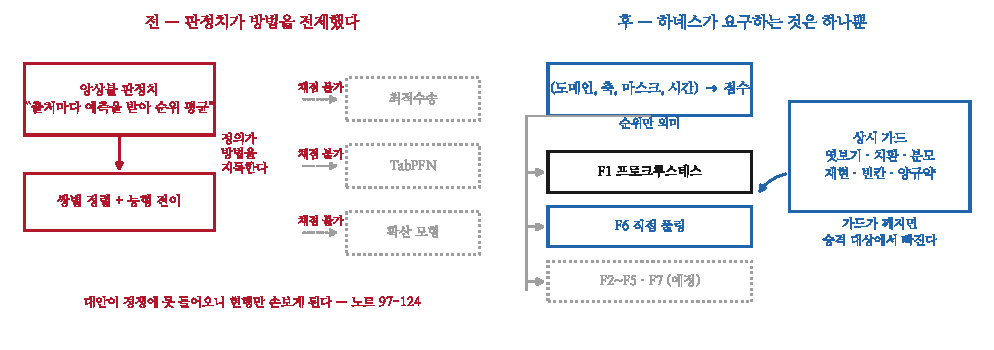
\includegraphics[width=\textwidth]{figs/lab.pdf}
\caption{왼쪽 --- 판정치의 정의가 방법을 지목하니 대안은 채점 자체가 안 됐다.
오른쪽 --- 하네스가 요구하는 것을 하나로 줄이고 가드를 상시화했다.}
\end{figure*}

\section{스물여덟 노트가 제자리를 돈 이유}

노트 97부터 124까지, 매 사이클이 ``후보 축을 하나 더 붙여 보고 채택 기준을
통과하나 본다''였다. 통과한 것은 노트 108 하나($+$0.4038 $\to$ $+$0.4270).
나머지는 전부 반증이었고, 반증 자체는 값진 것이었지만 \textbf{탐색 반경이
한 번도 안 커졌다.}

이유가 취향이나 게으름이 아니었다. 판정치의 정의에 있었다.

\claimx{\textbf{``앙상블 판정치''는 방법을 전제한 정의였다.} 대상마다 들어오는
출처 예측을 순위 평균한 뒤 스피어만 --- 이 문장은 \emph{출처가 여럿이고 각각
대상으로 전이된다}는 구조를 이미 가정한다. 전이 구조가 없는 정식화(단일 결합
모형, in-context 추론, 동역학 모형)는 ``출처별 예측''이라는 항 자체가 없어서
점수를 낼 수 없다.}{정의가 방법을 가둔다는 진단은 사후적이다. 처음부터 그렇게
설계한 것이 아니라 노트 5의 편의가 40편의 제약이 됐다.}

그래서 정식화에 요구하는 것을 하나로 줄였다.
\[
  (d,\; \mathbf{A},\; \mathbf{M},\; \mathbf{t}) \;\longmapsto\; \mathbf{s}\in\mathbb{R}^{n},
  \qquad \text{순위만 의미}
\]
$\mathbf{A}$는 축 행렬, $\mathbf{M}$은 관측 마스크, $\mathbf{t}$는 시간이다.
이 인터페이스만 지키면 무엇이든 붙는다. 현행 파이프라인도 여기서는 구현 하나다.

\section{상시 가드 --- 그리고 내가 처음 틀린 방식}

노트 87 · 115 · 117 · 124는 전부 내가 낸 수치를 내가 뒤집은 사건이었고,
공통 신호는 ``수치가 이상하다''가 아니라 \textbf{``수치가 너무 깔끔하다''}
였다. 세 번 다 논문을 내보낸 \emph{뒤에} 잡았다. 그래서 검사를 실행 시점으로
옮겼다.

\begin{table}[t]
\centering\tsize
\caption{모든 실행에 자동으로 붙는 가드. 깨지면 점수는 남되 승격 대상에서 빠진다.}
\begin{tabular}{ll}
\toprule
엿보기 & 대상 라벨을 섞어도 예측이 불변해야 \\
치환 & 출처 라벨을 섞으면 무너져야 (귀무 99회) \\
분모 & 대상 집합이 기준과 같아야 (노트 82 · 90) \\
재현 & 씨앗 넷의 폭 \\
빈칸 & 축이 전부 상수인 레코드 비중 (노트 124) \\
양규약 & 배포 대 전체의 낙관 편의 (노트 112) \\
\bottomrule
\end{tabular}
\end{table}

첫 판에서 치환 가드가 F1과 F6을 둘 다 떨어뜨렸다. F1은 라벨을 섞고도 팝업
$\rho$ $+$0.4929, F6은 $+$0.2322였다. ``신호의 90\%가 라벨에서 오지
않는다''고 읽을 뻔했다.

\claimx{\textbf{틀린 것은 결과가 아니라 검사였다.} 한 번 섞어 한 값을 보고
판정했는데, 그 값은 귀무의 \emph{평균}이 아니라 \emph{한 표본}이다. 99번
섞으니 팝업 귀무는 평균 $\approx$0, \textbf{표준편차 $\pm$0.35}(F1) ·
$\pm$0.26(F6)이다. 내가 뽑은 $+$0.49는 그 분포의 위쪽 꼬리였다.}{R=99는
$p$의 최소 해상도가 0.01이다. 더 촘촘한 판정이 필요하면 R을 올려야 한다.}

\begin{figure*}[t]
\centering
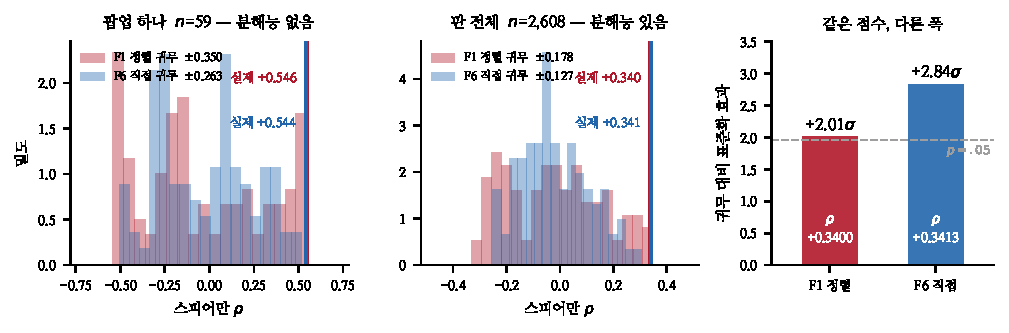
\includegraphics[width=\textwidth]{figs/null.pdf}
\caption{왼쪽 --- 팝업 하나의 귀무 폭이 $\pm$0.26$\sim$0.35다. 실제값
$+$0.54가 귀무의 1.5$\sim$2.1 표준편차 밖에 불과하다. 가운데 --- 판 전체로
모으면 귀무가 좁아진다. 오른쪽 --- 원점수는 무승부인데 표준화하면 갈린다.}
\end{figure*}

\section{대표 수치 자리에 분해능이 없었다}

팝업은 제품이 묻는 자리라 대표 수치로 써 왔다. 그런데 배포 규약에서 팝업의
후행 표본은 \textbf{59건}이다.

\claimx{\textbf{팝업 단독 $\rho$의 절대값은 정식화를 가르지 못한다.} 무작위
라벨로 적합한 예측도 $|\rho|$ 0.5를 예사로 낸다(귀무 폭 $\pm$0.26$\sim$0.35).
실제 $+$0.54는 그 안에서 1.5$\sim$2.1$\sigma$ 자리다.}{\textbf{과거의 채택
결정이 잡음이었다는 뜻은 아니다.} 노트 82 이후의 채택 기준은 절대값이 아니라
\emph{같은 표본에 짝지은 차이}의 붓스트랩이었고, 짝짓기는 공통 분산을 상쇄해
훨씬 좁다(노트 123의 구간 법칙 $2.28\,n^{-0.88}$, $n$=59에서 0.063). 잘못된
것은 절대값을 \emph{순위표의 대표 수치}로 쓴 것이다.}

그래서 순위 기준을 대상 하나에서 판 전체로 옮겼다. 대상별 $\rho$를 채점
표본 수로 가중 평균하면 $n$=2{,}608이고, 여기에 치환 귀무를 세워 표준화한다.
\[
  z \;=\; \frac{\bar\rho_{\text{실제}} - \operatorname{E}[\bar\rho_{\pi}]}
                {\operatorname{sd}[\bar\rho_{\pi}]}
\]

\section{첫 라운드 --- 챔피언이 바뀌었다}

포트폴리오에 셋을 올렸다. F0 무작위(바닥선), F1 프로크루스테스(노트 5--124의
파이프라인), F6 직접 풀링(정렬을 아예 안 하고 전 도메인을 한 표에 쌓은 뒤
도메인 표시자와 관측 표시자만 준다).

\begin{table}[t]
\centering\tsize
\caption{배포 규약, $T$=2025.0. 출처는 2025년 이전, 대상은 이후.
팝업은 2025년 이전 표본이 16건뿐이라 \textbf{어느 쪽도 팝업 과거를 학습하지
않는다} --- 순수 교차 도메인 비교다.}
\begin{tabular}{lrrrr}
\toprule
& 판 $\rho$ & 귀무 폭 & $z$ & 대상 \\
\midrule
F6 직접 풀링 & $+$0.3413 & 0.127 & $\mathbf{+2.84}$ & 9 \\
F1 프로크루스테스 & $+$0.3400 & 0.178 & $+$2.01 & 8 \\
F0 무작위 & $+$0.0041 & --- & --- & 9 \\
\bottomrule
\end{tabular}
\end{table}

\claimx{\textbf{정렬 기구는 원점수를 사지 못한다.} 겹치는 여덟 대상에서
F6 $+$0.3435, F1 $+$0.3399다. 도메인별로 보면 F6이 게임에서 $+$0.171
크게 이기고 나머지 일곱에서 $-$0.003$\sim$$-$0.047 작게 진다.}{한 시간
분할($T$=2025.0) 한 판이다. 분할을 옮기면 순서가 바뀔 수 있다.}

\claimx{\textbf{그리고 F1은 아이돌을 채점하지 못한다.} 완전사례 필터가
25건 중 18건만 남겨 최소 표본 20건을 못 채운다. 분모 가드가 이걸 잡았다
--- F1의 대상은 8개, 기준은 9개다.}{분모 불일치는 승격 자격 박탈 사유지
성능 판정이 아니다. 여덟 대상만으로 비교해도 결론은 같다.}

\begin{figure*}[t]
\centering
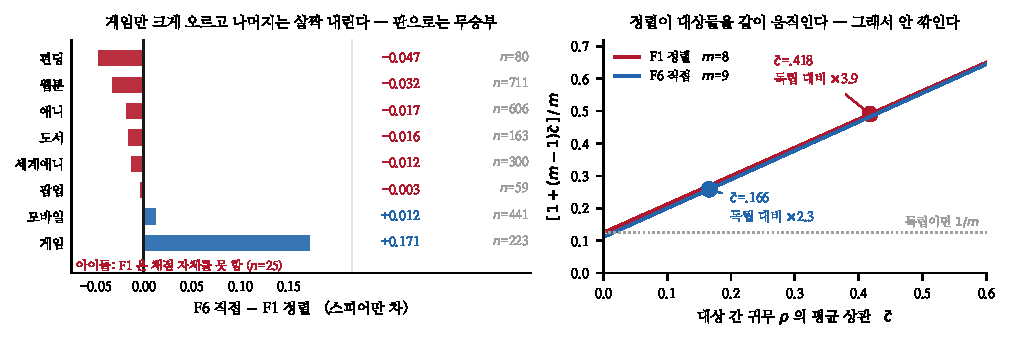
\includegraphics[width=\textwidth]{figs/flip.pdf}
\caption{왼쪽 --- 도메인별 대결. 오른쪽 --- 귀무 폭 차이의 기제.}
\end{figure*}

\section{정렬이 산 것은 자유도였다}

원점수가 같은데 귀무 폭이 1.41배 다르다. 왜인가.

먼저 아닌 것부터. 정렬이 출처들의 \emph{오차}를 묶었을 것이라 짐작했는데
틀렸다. 실제 라벨에서 아홉 출처의 예측은 서로 $\bar c$ $=$ $+$0.807로
붙어 있지만, \textbf{치환 라벨에서는 $-$0.001로 독립}이다. 출처들이 붙는 건
공유 신호 때문이지 기구 때문이 아니다. (이 $+$0.807은 노트 119--121이
곡선 적합으로 얻은 $\bar c\approx0.82$를 전혀 다른 경로로 재확인한다.)

기제는 한 층 위에 있었다.

\claimx{\textbf{치환 라벨에서 F1은 대상들을 같이 움직인다.} 대상별 귀무
$\rho$의 쌍 상관이 F1 $+$0.418(96\%가 양수), F6 $+$0.166(69\%)이다. 프로크루스테스가
모든 대상을 하나의 정렬된 잠재 공간으로 밀어 넣으니, 무작위 능형 방향
하나가 대상 전체를 같은 쪽으로 기울인다. F6은 도메인 표시자가 그 이동을
흡수한다.}{$\bar c$는 99회 치환에서 잰 것이고 표본 오차가 있다.}

이것을 앙상블 분산식에 넣으면 판 통계량의 폭이 나온다.
\[
  \operatorname{Var}(\bar\rho) \;\approx\; \frac{\sigma^{2}}{m}\bigl[\,1+(m-1)\bar c\,\bigr]
\]
F1은 $m$=8, $\bar c$=0.418이라 독립 대비 3.9배, F6은 $m$=9, $\bar c$=0.166이라
2.3배다. 대상별 귀무 폭의 평균($\sigma$: F1 0.256, F6 0.213)을 곱하면
예측 폭이 F1 \textbf{0.179} · F6 0.108이고, 실측은 F1 \textbf{0.178} ·
F6 0.127이다.

\claimx{\textbf{정렬은 적합도를 사지 않고 자유도를 샀다.} 같은 원점수를 내는데
우연히 그 점수를 낼 길이 두 배 가까이 많다. 어떤 간결성 기준으로 보아도
F1은 F6보다 나쁜 모형이다.}{F1 예측(0.179 대 0.178)은 거의 정확하지만
F6은 17\% 어긋난다 --- 판 평균이 표본 수 가중인데 식은 비가중이라 생기는
근사 오차로 본다. 정확한 가중 형태는 아직 안 유도했다.}

\section{무엇이 바뀌고 무엇이 그대로인가}

바뀐 것은 루프의 크기다. 이제 사이클은 ``F1을 개선한다''가 아니라
\textbf{``도전자를 챔피언에 붙이고, 이기면 승격 지면 은퇴''}다. 고정된 것은
목표(IP · 기획 $\to$ 소비자 반응)와 하네스뿐이고, 세부 계획은 매 사이클
바뀌어도 된다.

실행은 전부 SQLite에 남고 별도 서버의 모니터가 읽는다
(\texttt{lab/server.py}, 포트 7801, 표준 라이브러리만). 한 라운드가 8초다
--- 세 정식화 $\times$ (두 규약 $+$ 가드 여섯 $+$ 붓스트랩 200회).

\begin{table}[t]
\centering\tsize
\caption{다음 도전자. 전부 같은 하네스로 채점된다.}
\begin{tabular}{ll}
\toprule
F2 & 결합 위계 잠재 모형 ($\tau$ 풀링, 우도 결측) \\
F3 & Gromov--Wasserstein --- 정렬 전제 자체를 제거 \\
F4 & TabPFN / CARTE --- in-context 베이즈 \\
F5 & 확산 --- 일자별 곡선 89개에서 $M,p,q$ 세 라벨 \\
F7 & anchor regression --- 불변 방향만 \\
\bottomrule
\end{tabular}
\end{table}

그대로인 것도 적어 둔다. \textbf{표본이 늘지 않았다.} 팝업 후행 59건은
그대로고, 귀무 폭 $\pm$0.26은 정식화를 바꿔서 줄일 수 있는 양이 아니다.
노트 124가 연 길 --- 축이 빈 260건을 매기면 팝업이 75건에서 322건이 된다
--- 이 여전히 이 판에서 제일 큰 한 수다. 하네스가 바뀌었으니 그 작업의
값어치는 오히려 더 커졌다. 어느 정식화가 이기든 같은 표본을 나눠 쓴다.

\end{document}
